\documentclass[12pt,titlepage]{article}
\usepackage[margin=1.25in]{geometry}
\usepackage{graphicx,amsmath,minted}

%% Variables definition
\newcommand{\vSubject}{Data Structure and Algorithm Practicum}
\newcommand{\vSubtitle}{Quiz 2}
\newcommand{\vName}{Dicha Zelianivan Arkana}
\newcommand{\vNIM}{2241720002}
\newcommand{\vClass}{1i}
\newcommand{\vDepartment}{Information Technology}
\newcommand{\vStudyProgram}{D4 Informatics Engineering}

%% [START] Tikz related stuff
\usepackage{tikz}
\usetikzlibrary{svg.path,calc,shapes.geometric,shapes.misc}
\tikzstyle{terminator} = [rectangle, draw, text centered, rounded corners = 1em, minimum height=2em]
\tikzstyle{preparation} = [chamfered rectangle, chamfered rectangle sep=0.75em, draw, text centered, minimum height = 2em]
\tikzstyle{process} = [rectangle, draw, text centered, minimum height=2em]
\tikzstyle{decision} = [diamond, aspect=2, draw, text centered, minimum height=2em]
\tikzstyle{data}=[trapezium, draw, text centered, trapezium left angle=60, trapezium right angle=120, minimum height=2em]
\tikzstyle{connector} = [line width=0.25mm,->]
%% [END] Tikz related stuff

%% [START] Fancy header related stuff
\usepackage{fancyhdr}
\pagestyle{fancy}
\setlength{\headheight}{15pt} % compensate fancyhdr style
\fancyhead{}
\fancyfoot{}
\fancyfoot[L]{\thepage}
\fancyfoot[R]{\textit{\vSubject - \vSubtitle}}
\renewcommand{\footrulewidth}{0.4pt}% default is 0pt, overline for footer
%% [END] Fancy header related stuff

%% [START] Custom tabular command related stuff
\usepackage{tabularx}
\newcommand{\details}[2]{
    #1 & #2  \\
}
%% [END] Custom tabular command related stuff

%% [START] Figure related stuff
\newcommand{\image}[3][1]{
    \begin{figure}[h]
        \centering
        \includegraphics[#1]{#2}
        \caption{#3}
        \label{#3}
    \end{figure}
}
%% [END] Figure related stuff

\begin{document}
\begin{titlepage}
    \centering
    \vfill
    {\bfseries\LARGE
        \vSubject\\
        \vskip0.25cm
        \vSubtitle
    }
    \vfill
    
\includegraphics[width=6cm]{images/polinema-logo.png}
    \vfill
    {
        \textbf{Name}\\
        \vName\\
        \vskip0.5cm
        \textbf{NIM}\\
        \vNIM\\
        \vskip0.5cm
        \textbf{Class}\\
        \vClass\\
        \vskip0.5cm
        \textbf{Department}\\
        \vDepartment\\
        \vskip0.5cm
        \textbf{Study Program}\\
        \vStudyProgram
    }
\end{titlepage}

\section{Questions}
\begin{enumerate}
    \item {
        Complete the \texttt{addLast()} and \texttt{deleteLast()} method inside the class\\
        \texttt{SingleLinkedList}

        \begin{itemize}
            \item {
                \texttt{addLast()}
                \begin{minted}[autogobble,fontsize=\small]{java}
                    void addLast(int data) {
                        // create a new node
                        Node newNode = new Node(data);
                        // checks if it's empty, meaning that we don't have any node yet
                        // so just assign the head and tail to the new node
                        if (isEmpty()) {
                            head = tail = newNode;
                        } else {
                            // otherwise, let's insert the new node into the next pointer of the tail
                            tail.next = newNode;
                            // and then replace the tail with our node
                            tail = newNode;
                        }
                        // increment the size
                        size++;
                    }
                \end{minted}
            }
            \item {
                \texttt{deleteLast()}
                \begin{minted}[autogobble,fontsize=\small]{java}
                    void deleteLast() {
                        Node tmp = head;
                        // traverse through the entire list until second to last
                        while (tmp.next.next != null) {
                            tmp = tmp.next;
                        }
                        // replace the tail with the second to last node
                        tail = tmp;
                        // remove the last node using the next pointer from the second to last node
                        tail.next = null;
                        // decrement the size
                        size--;
                    }
                \end{minted}
            }
        \end{itemize}
    }
    \pagebreak
    \item {
        Complete the method \texttt{merge()} and \texttt{split()} inside the method \texttt{Main}

        \begin{itemize}
            \item {
                \texttt{merge()}
                \begin{minted}[autogobble,fontsize=\small]{java}
                    public static void merge(SingleLinkedList l1, SingleLinkedList l2) {
                        SingleLinkedList mergedList = new SingleLinkedList();

                        // insert every nodes from the first list into the merged list
                        Node current = l1.head;
                        while (current != null) {
                            // use addLast to insert it consecutively in order
                            // instead of in reverse order
                            mergedList.addLast(current.data);
                            // traverse to the next node
                            current = current.next;
                        }

                        // do the same thing with the second node
                        current = l2.head;
                        while (current != null) {
                            mergedList.addLast(current.data);
                            current = current.next;
                        }

                        // just to proof the list has been merged
                        System.out.print("Merged List: ");
                        mergedList.print();
                    }
                \end{minted}
            }
            \item {
                \texttt{split()}
                \begin{minted}[autogobble,fontsize=\small]{java}
                    public static void split(SingleLinkedList list) {
                        // prepare 2 lists that will be used to contain our split list
                        SingleLinkedList firstList = new SingleLinkedList();
                        SingleLinkedList secondList = new SingleLinkedList();

                        // get the middle point since we're going to split it by half
                        int middle = list.size / 2;

                        // split the first portion into the first list
                        Node current = list.head;
                        // loop until we reach the half point
                        for (int i = 0; i < middle; i++) {
                            // again, we want to insert it in order so we'll use 
                            // addLast instead of addFirst
                            firstList.addLast(current.data);
                            current = current.next;
                        }

                        // do the same thing but for the last portion of the list
                        current = list.head;
                        // we start from the middle until the last part of the list
                        // which is equal to the list.size
                        for (int i = middle; i < list.size; i++) {
                            secondList.addLast(current.data);
                            current = current.next;
                        }

                        System.out.println("Split list: ");

                        // just to proof that the list has been split
                        System.out.print("First List: ");
                        firstList.print();

                        // do the same for the second list
                        System.out.print("Second List: ");
                        secondList.print();
                    }
                \end{minted}
            }
        \end{itemize}
    }
\end{enumerate}

\section{Solution Source Code}
See the attached files

\section{Screenshots}
\begin{figure}[h]
    \centering
    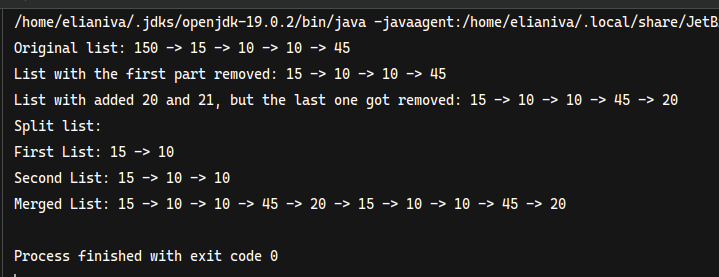
\includegraphics[width=\textwidth]{./images/output.png}
    \caption{The output of the program when ran from \texttt{Main.java}}
\end{figure}

\end{document}

